\begin{frame}
    \frametitle{Cámara Time of Flight}
    \note{https://en.wikipedia.org/wiki/Time-of-flight_camera}
    \tiny
    \begin{center}
        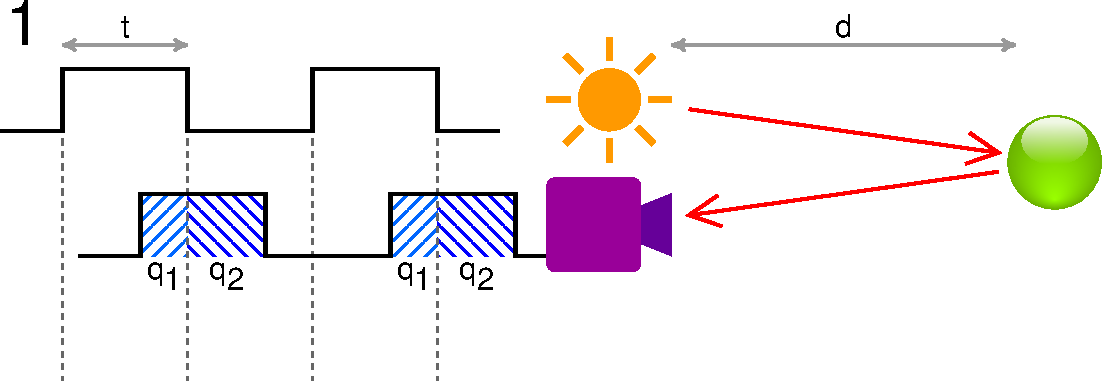
\includegraphics[width=0.3\columnwidth]{images/time_of_flight_camera_pulse.pdf}
        \hspace{3em}
        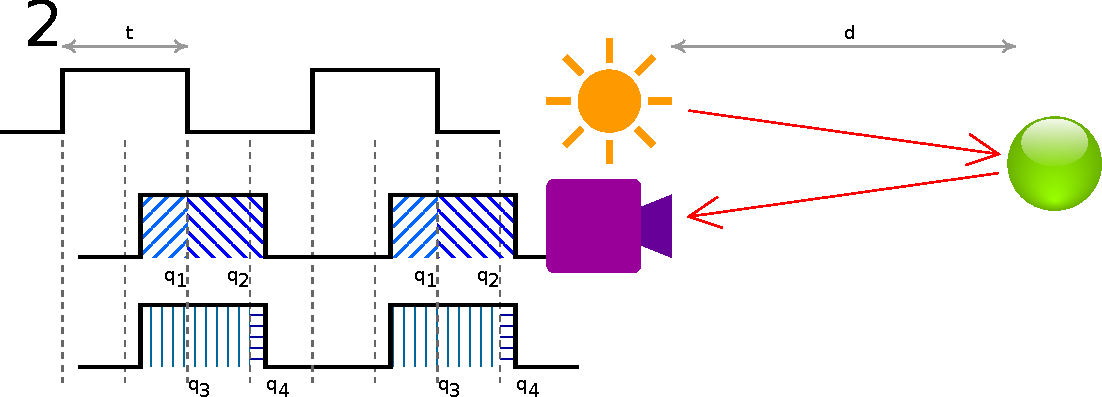
\includegraphics[width=0.3\columnwidth]{images/time_of_flight_camera_continuous_wave.pdf}
    \end{center}

    \begin{block}{Principio de funcionamiento}
        Funciona de manera similar a un LiDAR con la ventaja de que toda la escena 3D se captura al mismo tiempo y que no hay partes móviles. Este dispositivo utiliza una fuente de luz infrarroja modulada para determinar la distancia en cada píxel de un sensor \emph{Photonic Mixer Device} (PMD).
        
        En el método basado en Pulsos (1), la ditancia es
        \begin{equation*}
            d = \dfrac{c t}{2} \dfrac{q_{2}}{q_{1} + q_{2}}
        \end{equation*}
        donde
        \begin{itemize}
            \item $c$ es la velocidad de la luz
            \item $t$ es la longitud del pulso
            \item $q_{1}$ es la carga acumulada en el píxel cuando se emite luz
            \item $q_{2}$ es la carga acumulada cuando no se emite
        \end{itemize}
        
        En el método de onda continua (2):
        \begin{equation*}
            d = \dfrac{c t}{2\pi} \arctan \dfrac{q_{3} - q_{4}}{q_{1} - q_{2}}
        \end{equation*}        
    \end{block}
    
    \begin{itemize}
        \item Esteroceptivo
        \item Activo
        \item La precisión suele estimarse en un $\SI{1}{\percent}$ de la distancia medida, suelen tener un frame rate de unos $\SI{160}{\hertz}$
        \item La luz del entorno puede quemar la imagen (requiere píxeles con buen rango dinámico)
    \end{itemize}
    
\end{frame}